\documentclass[a4paper,12pt]{article}

\usepackage[utf8]{inputenc}
\usepackage[T1]{fontenc}
\usepackage{graphicx}
\usepackage{color}
\usepackage{amsmath}
\usepackage{amsfonts}
\usepackage{amssymb}
\usepackage{multicol}
\usepackage{eurosym}
\usepackage{bbm}
\usepackage[french]{babel}
\usepackage{lastpage}
\usepackage{float}
\usepackage{upgreek}
\usepackage{verbatim}
\usepackage{moreverb}
\usepackage{listings}
\usepackage{textcomp}
\usepackage[nottoc]{tocbibind}
\usepackage{hyperref}
%\usepackage{subfigure}
\usepackage{subcaption}

\usepackage{etoolbox}

%%%Package Cedric
\usepackage[table,xcdraw]{xcolor}

\definecolor{color_caption}{rgb}{0.3,0.3,0.3}
\definecolor{color_section}{rgb}{0.9,0,0}
\definecolor{em_orange}{rgb}{0.9686,0.5765,0.1137}
\definecolor{em_pink}{rgb}{0.9294,0.0078,0.5490}
\definecolor{em_blue}{rgb}{0.1412,0.6667,0.8824}
\definecolor{em_green}{rgb}{0.5451,0.7765,0.2431}

\usepackage{caption}
\usepackage[font={color=color_caption},figurename=Figure,labelfont={it}]{caption}

\lstset{
language=C,basicstyle=\normalsize,upquote=true,aboveskip={1.5\baselineskip},columns=fullflexible,showstringspaces=false,extendedchars=true,breaklines=true,showtabs=false,showspaces=false,showstringspaces=false,identifierstyle=\ttfamily,keywordstyle=\color[rgb]{0,0,1},commentstyle=\color[rgb]{0.133,0.545,0.133},stringstyle=\color[rgb]{0.627,0.126,0.941},}

\DeclareMathOperator{\G}{G}

\renewcommand{\arraystretch}{1.5}
\renewcommand{\baselinestretch}{1.5}

\textheight 255mm
\headheight 15mm
\oddsidemargin -10mm
\evensidemargin -10mm
\marginparwidth 5mm
\topmargin -20mm
\textwidth 185mm
\headsep 5mm
\footskip 10mm


\usepackage{fancyhdr}

\pagestyle{fancy}

\renewcommand{\headrulewidth}{2pt}
\renewcommand{\headrule}{\hbox to\headwidth{\color{em_orange}\leaders\hrule height \headrulewidth\hfill}}
\fancyhead[L]{ENSEIRB-MATMECA}
\fancyhead[C]{Projet avancé SE}
\fancyhead[R]{E3}

\renewcommand{\footrulewidth}{2pt}
\patchcmd{\footrule}{\hrule}{\color{em_orange}\hrule}{}{}
\fancyfoot[C]{\thepage}

\usepackage{eso-pic}
\newcommand\BackgroundPic{%
\put(0,0){%
\parbox[b][\paperheight]{\paperwidth}{%
\vfill
\centering

\includegraphics[scale=0.6,%
keepaspectratio]{background}%
\vfill
}}}


\begin{document}
\parindent=1cm
\everymath{\displaystyle}
%
\AddToShipoutPicture*{\BackgroundPic}
%
\thispagestyle{empty}
%
%
\noindent
Cédric DUMONDELLE\hfill{E3}\\
Lucas FILLON\\
Xavier MARINO\\
Pierre OLIVIER\\
%
\\
%
\vspace{5.5cm}
{\color{white}t}\\
%
{\color{em_orange}\rule{\linewidth}{2pt}}
%
\textbf{{
\begin{center}
\Huge Projet avancé SE\\
%\vspace{0.6cm}
\end{center}
}}
%
{\color{white}t}\\
{\color{em_orange}\rule{\linewidth}{2pt}}\\

\vspace{9.5cm}

%
Yannick BORNAT \& Bertrand LE GAL
% \begin{tabular}{rcl}
% Dominique Dallet\hspace{4cm}\vphantom{e}&
% Professor Izzet Kale\hspace{4cm}\vphantom{e}&
% Saumya Reni
% \end{tabular}
% %
\ClearShipoutPicture
%
\newpage
%
\thispagestyle{empty}
\tableofcontents
%
\newpage
%%%%%%%%%%%%%%%%%%%%%%%%%%%%%%%%%%%%%%%%%%%%%%%%%%%%%
\setcounter{section}{-1}
\section{Introduction}
\subsection{Contexte}
\subsection{Problématique}
\newpage
\section{Présentation du cas d'étude}
\subsection{Introduction}
Afin de mener à bien cette étude nous nou sommes basés sur les travaux de Yannick Bornat. En effet, dans le cadre de l'analyse de signaux biomédicaux, ce dernier a mis au point un module de détection d'activité de cellules biologique, en VHDL.\\

Dans le cas de signaux provenant de cellules biologiques, l'activité cellulaire peut être détectée par un pic d'amplitude, celui-ci est représenté en figure XX. Cependant ce type de signaux possède une composante en bruit basse fréquence très élevée, c'est pourquoi il doit être filtré en amont. C'est ce signal filtré qui est utilisé à la détermination d'une valeur de seuil nécessaire à la détection d'activité biologique. Ce principe de fonctionnement, qui sera à la base du développement de notre module, est illustré en figure XX.\\

\begin{figure}[H]
\centering
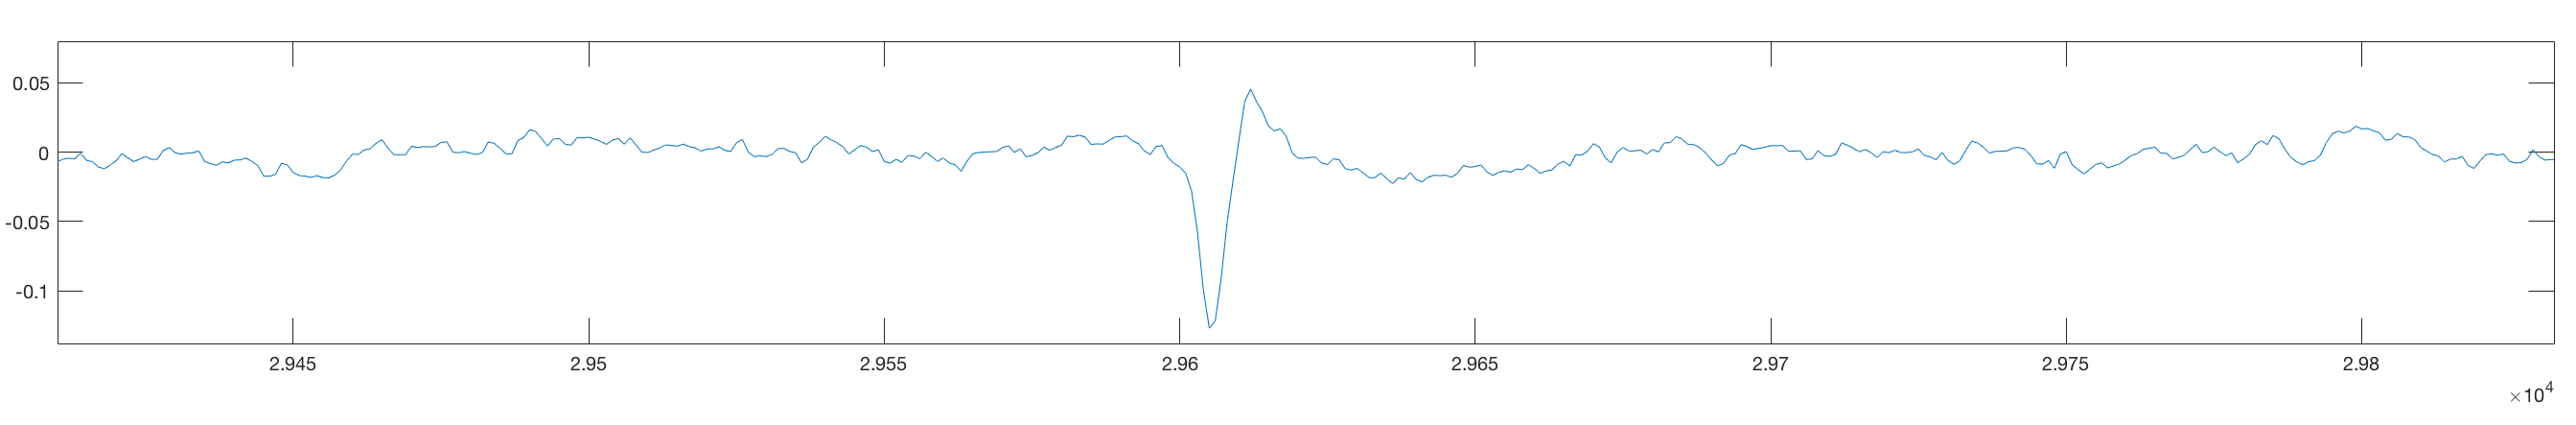
\includegraphics[scale=0.18, keepaspectratio]{toto3.png}
\caption{\textit{Pic d'activité dans un signal biologique}}
\end{figure}

\begin{figure}[H]
\centering
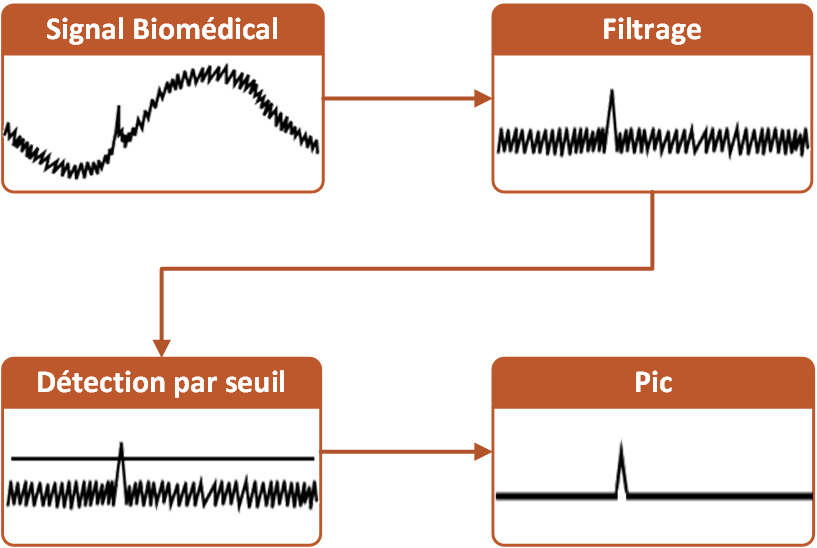
\includegraphics[scale=0.5, keepaspectratio]{Dessin1.png}
\caption{\textit{Principe de fonctionnement du module de détection d'activité cellulaire}}
\end{figure}
\newpage

\subsection{Fonctionnement des différents blocs}
Comme énoncé précédement, les signaux issus de capteurs biologiques sont très fortement bruité en basse fréquence, ceci se caractérise par une forte variation de l'amplitude du signal. Cette variation d'amplitude, illustrée en figure XX a) sur 5000 échantillons, est du même ordre, voir plus grand, que les que les pics attestants d'une activité celllulaire. Il convient donc de supprimer ce bruit afin de correctement détecter les pics d'activité.\\
\begin{itemize}
\item[•] \textbf{Suppression du bruit basse fréquence contenu dans le signal d'entré} : c'est un filtre à réponse impulsionnelle infinie (IIR) qui est utilisé pour s'affranchir des basses fréquence, suivant l'équation (1).
\begin{eqnarray}
y_n = \frac{63}{64}\left(x_n - x_{n-1}\right) + \frac{31}{32}y_{n-1}
\end{eqnarray}
Le résultat issus de cette première étape de filtrage est illustré en figure XX b), on retrouve les pics caractéristiques du signal, mais celui-ci est désormais centré sur 0. On peut, cependant, constater que ce signal est également bruité en haute fréquence. C'est pour limiter l'impact de ce bruit, qu'une valeur de seuil adaptative est utilisée afin détecter les pics.\\

\item[•] \textbf{Calcul de la valeur de seuil} : deux modèles différents ont été explorés lors de cette étape, l'un d'entre eux reprennant les travaux de Yannick Bornat en appliquant une boucle de correction sur le signal d'entré filtré, tandis que l'autre méthode utilise la valeur d'écart type, de nouveau appliqué au signal filtré, (à un facteur de proportionnalité près), comme valeur de seuil.\\
\newpage
\begin{itemize}
\item[\textbf{a)}] \textbf{Calcul du seuil par boucle de correction} :
	\begin{figure}[H]
		\centering
		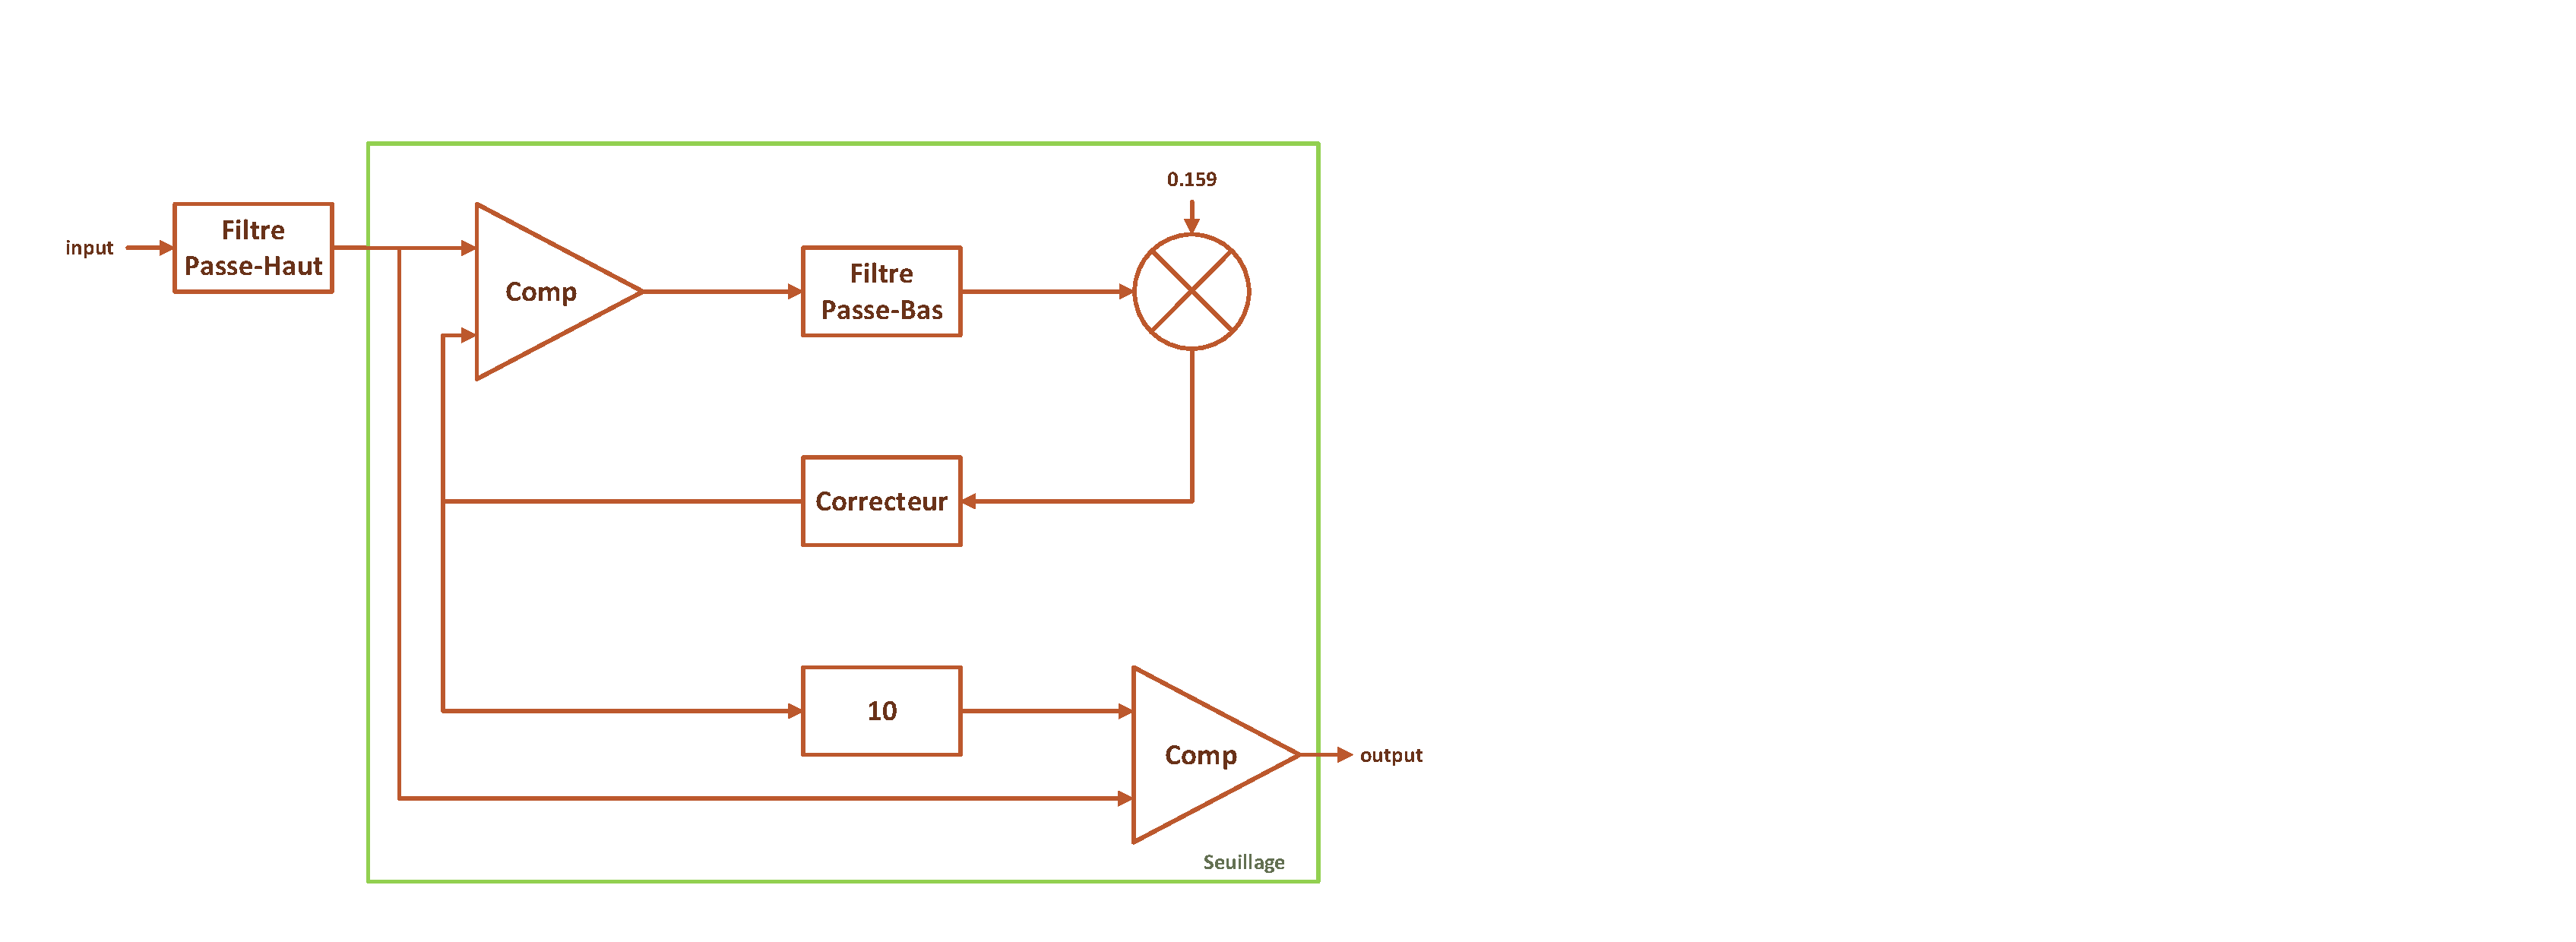
\includegraphics[scale=0.4, keepaspectratio]{chainCedric.pdf}
		\caption{Architecture du seuillage avec correcteur}
	\end{figure}
	Dans ce modèle, le but est de fixer le seuil de façon à ce qu'uniquement $15.9\%$ des échantillons soient supérieurs à celui-ci.
	Dans ce but, une boucle de contre-réaction est mise en place afin d'adapter la valeur de seuil afin de remplir cette condition.
	Dans un premier temps, l'échantillon est comparé avec la valeur de seuil actuelle. Le comparateur produira un niveau haut si celui-ci est supérieur au seuil et produira un niveau bas sinon. Le filtre passe-bas qui suit sert de moyenneur.
	En effet, celui-ci permet de calculer la valeur moyenne des sorties du comparateur sur un certain nombre d'echantillon.
	En d'autres termes, il donne en sortie le pourcentage d'echantillon au dessus de la valeur de seuil. Après soustraction de $0.159$, la valeur de sortie de ce moyenneur est envoyé en entrée du correcteur composé d'un proportionnel integrateur ce qui permet d'annuler l'erreur statique.
	Cette boucle de contre réaction permet la mise à jour perpetuelle de la valeur de seuil. Pour finir, les echantillons sont comparé à celle-ci multiplié par $10$ et le resultat de cette comparaison est envoyé en sortie. Ce résultat correspond à la présence (niveau haut) ou non (niveau bas) d'un pic.
	\newpage
	\item[\textbf{b)}] \textbf{Calcul du seuil par écart type} :
	\begin{figure}[H]
		\centering
		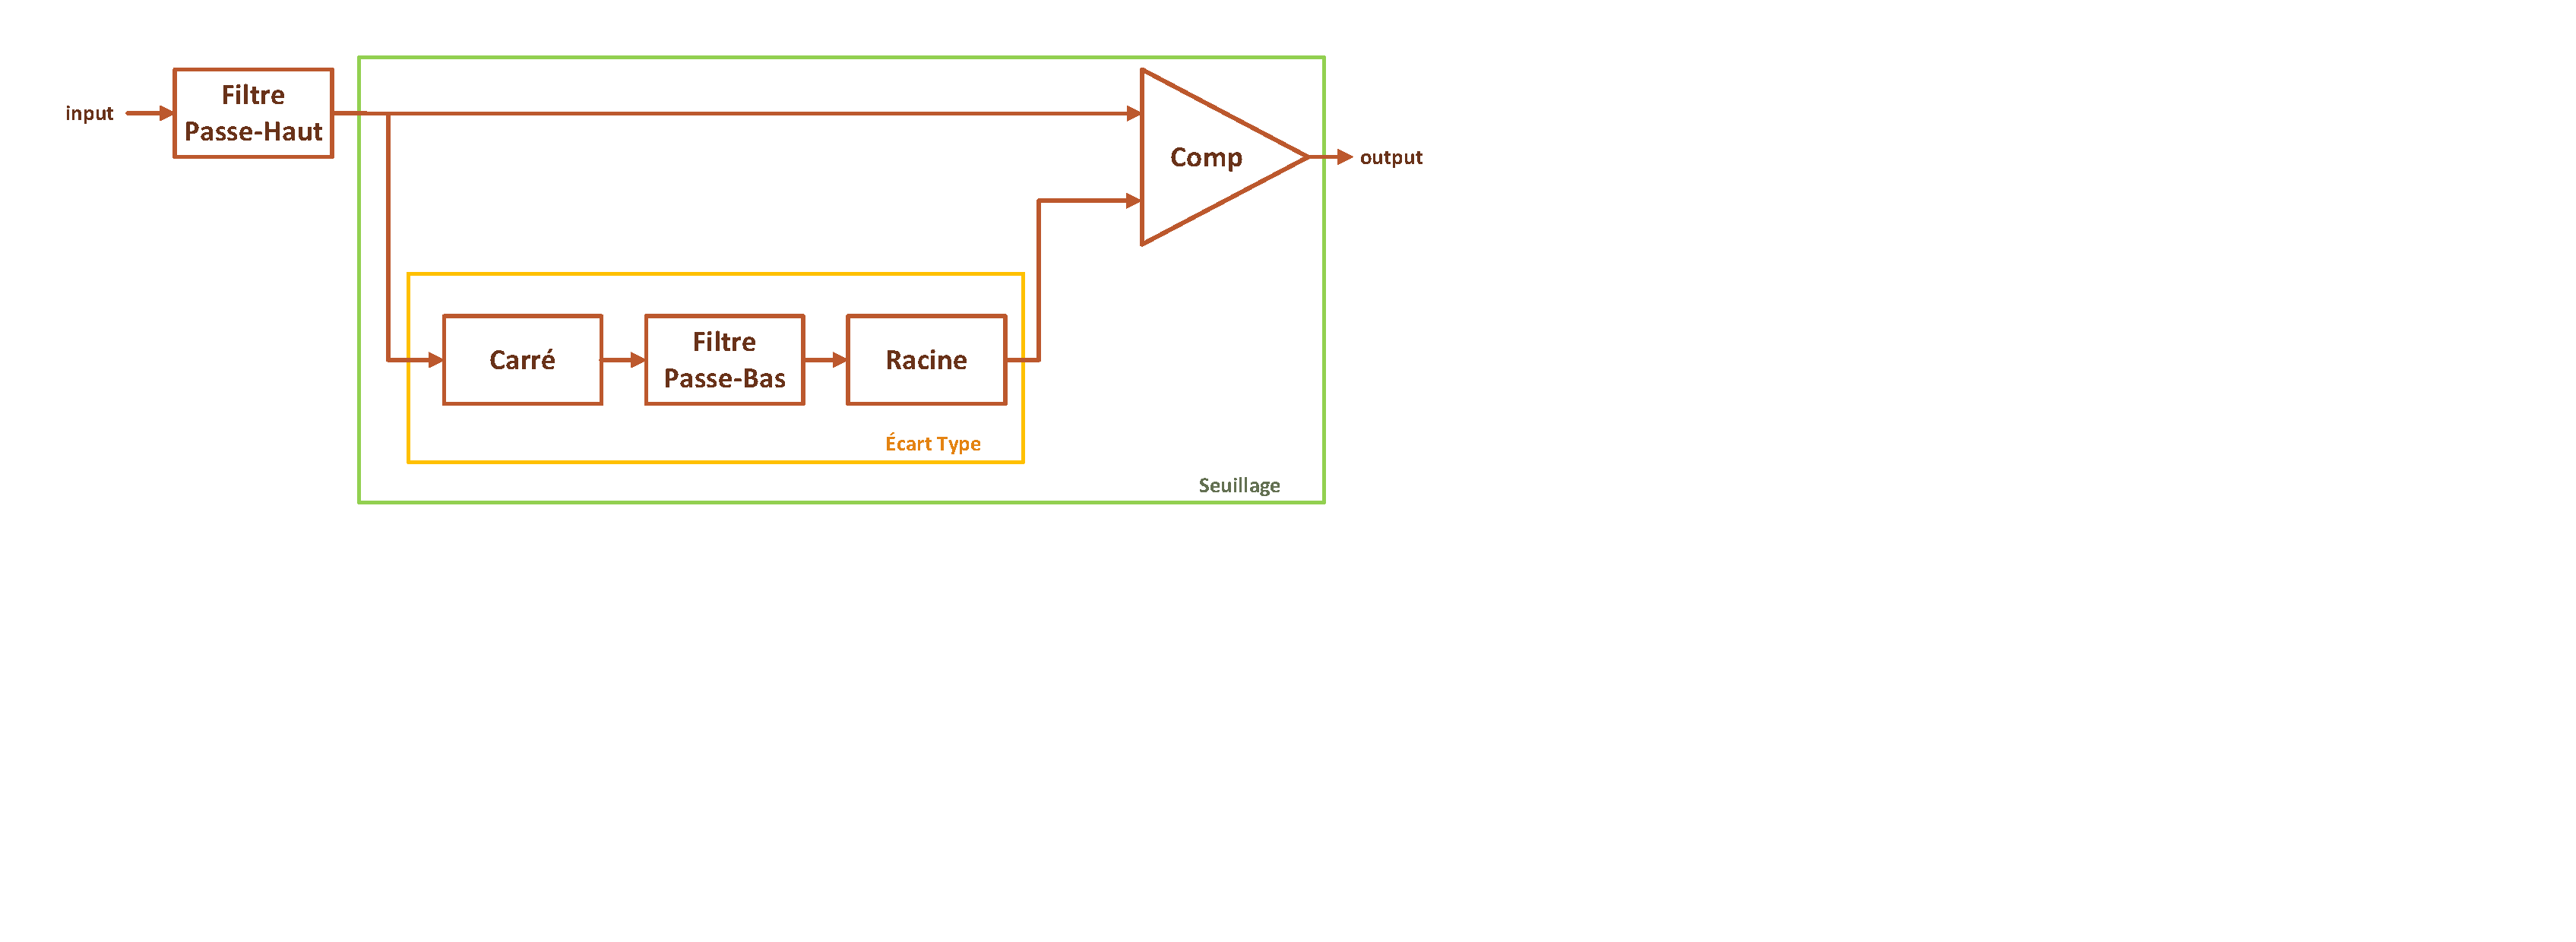
\includegraphics[scale=0.4, keepaspectratio]{chainXavier.pdf}
		\caption{Flot de compilation}
	\end{figure}
\end{itemize}
\end{itemize}
\begin{figure}[H]
\centering
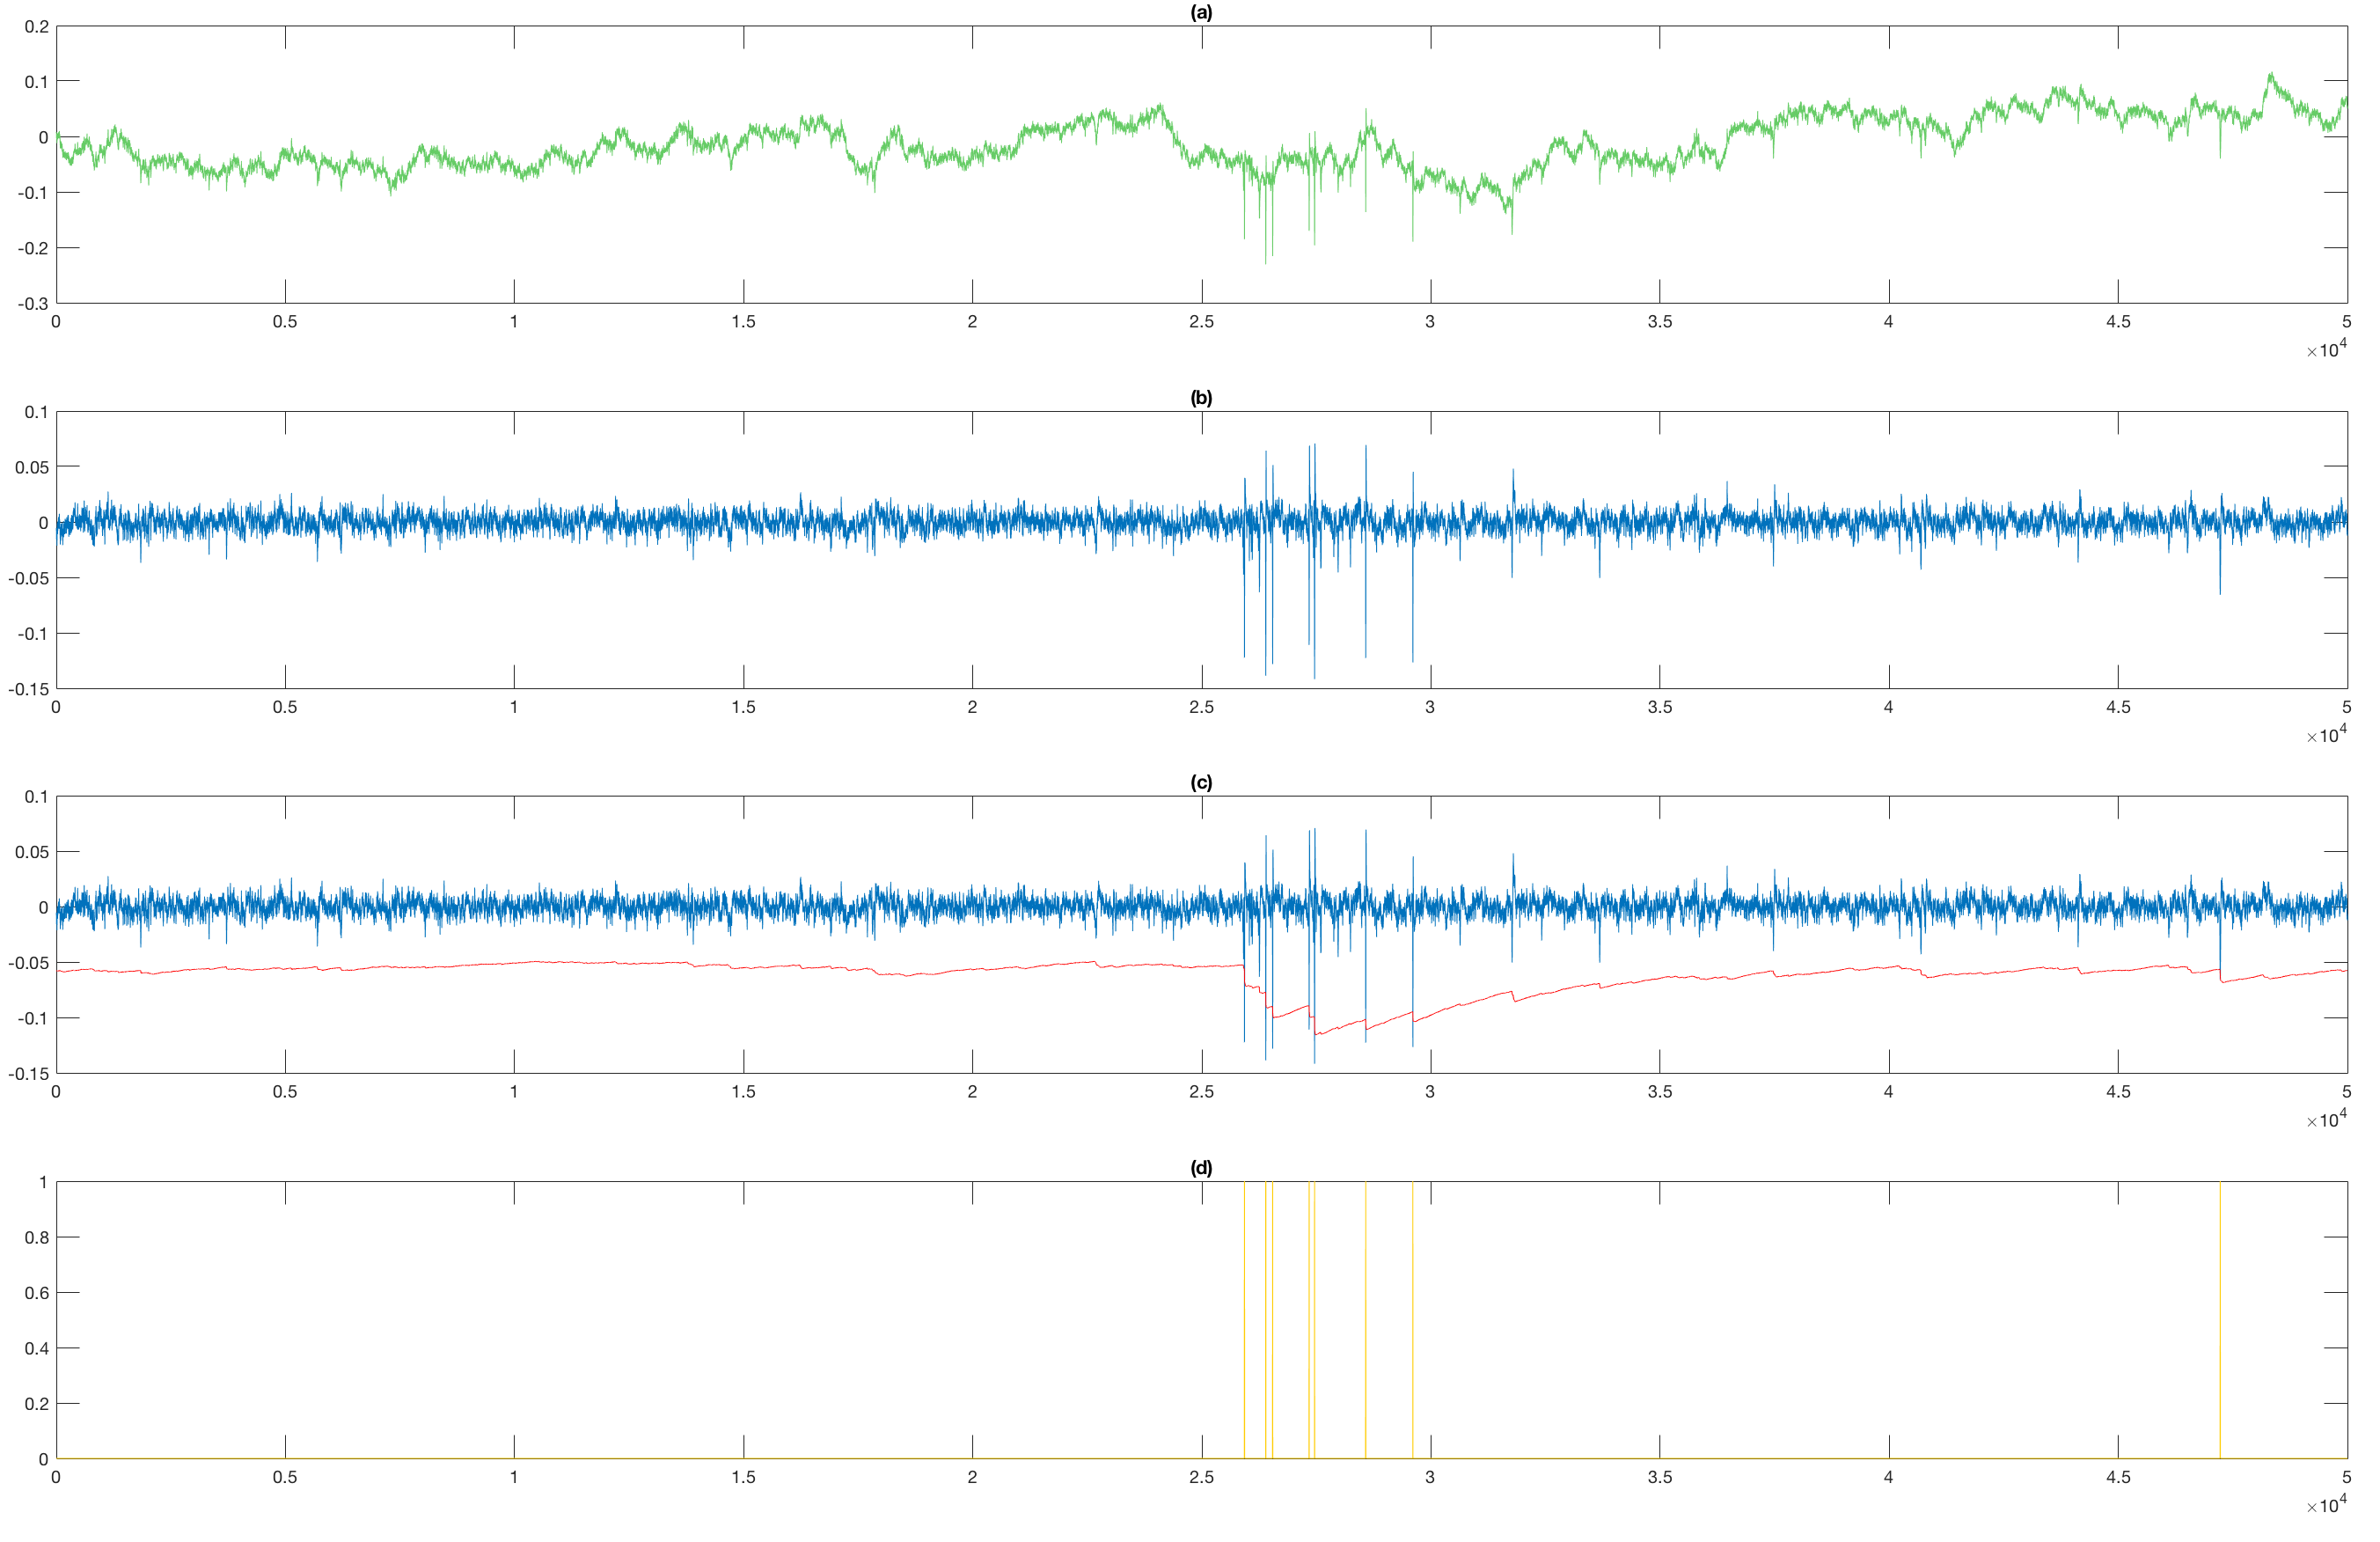
\includegraphics[scale=0.18, keepaspectratio]{toto2.png}
\caption{\textit{toto}}
\end{figure}
\newpage
\section{Implémentation depuis le SystemC}
	Les schémas présentés en Figures X et X permettent de se représenter le fonctionnement de la chaîne globale. La modularité du SystemC nous permet alors de concevoir une paire de fichiers, un fichier source de description ainsi qu'un \textit{header}, pour chacun des blocs composant ces schémas. Il convient de détailler le cheminement suivi à partir de la création de ces fichiers jusqu'à leur implémentation sur la carte Nexys 4. Cette partie vient donc présenter le flot de conception/compilation lié au SystemC et sa mise en oeuvre lors du projet.

\subsection{Flot de compilation}
	L'apprentissage d'un nouveau langage de description ou de programmation passe nécessairement par la compréhension du flot de compilation qui lui est associé. Pour le SystemC, on peut découper ce flot en quatre étapes principales illustrées par la Figure X :
	\begin{figure}[H]
		\centering
		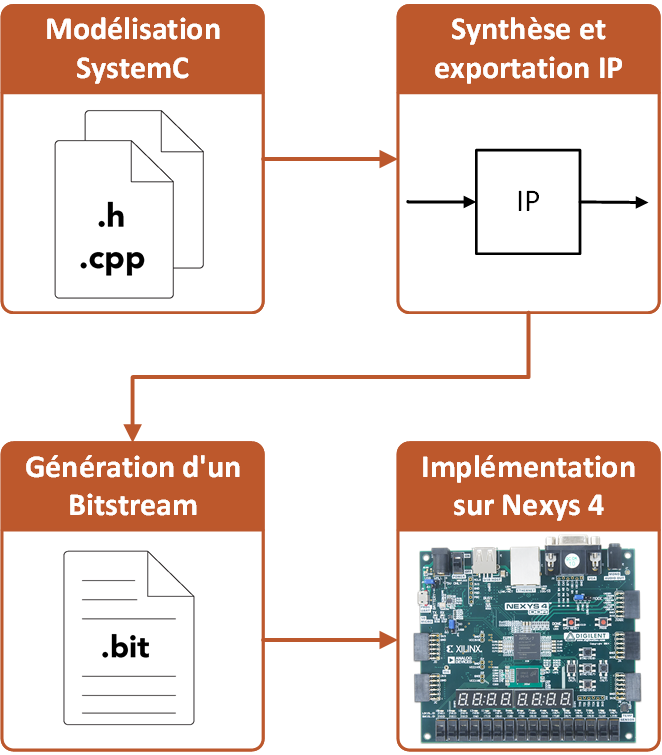
\includegraphics[scale=0.5, keepaspectratio]{Dessin2.png}
		\caption{Flot de compilation}
	\end{figure}
	\begin{itemize}
		\item[\textbullet] \textbf{Modélisation SystemC} : dans un premier temps il convient de décrire en SystemC le système que l'on souhaite modéliser. Pour cela, on rédige des fichiers sources dans un IDE SystemC pour symboliser chacun des blocs décrits précédemment. \\
		\item[\textbullet] \textbf{Synthèse et exportation IP} : une fois les fichiers SystemC écrits, on peut désormais les passer dans l'environnement \textit{Vivado HLS} afin de les synthéthiser et d'exporter un ou plusieurs blocs sous forme d'IP (\textit{Intellectual Property}). Ces blocs IP sont des blocs logiques, avec des entrées et des sorties, qui vont être implémentés sur FPGA par la suite. \\
		\item[\textbullet] \textbf{Génération d'un Bitsream} : un bloc IP ne pouvant être envoyé directement sur FPGA, il convient de l'intégrer dans un \textit{top-level}, décrit en langage VHDL, pour pouvoir notamment interfacer ses entrées et sorties avec les entrées et sorties physiques de la carte Nexys 4. Pour ce faire, l'environnement \textit{Vivado} est requis et permet de générer un \textit{bitsream} d'extension \texttt{.bit}. \\
		\item[\textbullet] \textbf{Implémentation sur Nexys 4} : finalement, le \textit{bitsream} peut être envoyé sur la carte cible, dans notre cas la carte Nexys 4, via le port série de notre ordinateur. A ce stade, les fichiers décrits en SystemC sont implémentés sur FPGA.\\
	\end{itemize}
	Le flot de compilation présenté ici allie le développement \textit{software} de sources SystemC, et l'implémentation \textit{hardware} des blocs ainsi créés. Il s'agit là du flot de compilation suivi lors du projet et les parties 2.2 et 2.3 suivantes viennent détailler sa mise en pratique.


\subsection{Modélisation en SystemC et simulations}
\subsection{Implémentation sur FPGA et validation}
	Une fois les fichiers SystemC écrits et les simulations en \textit{software} vérifiées, il convient de tester les blocs et chaînes entières en \textit{hardware}. Pour cela, un environnement de test a été mis en place et il est illustré en Figure X.
	\begin{figure}[H]
		\centering
		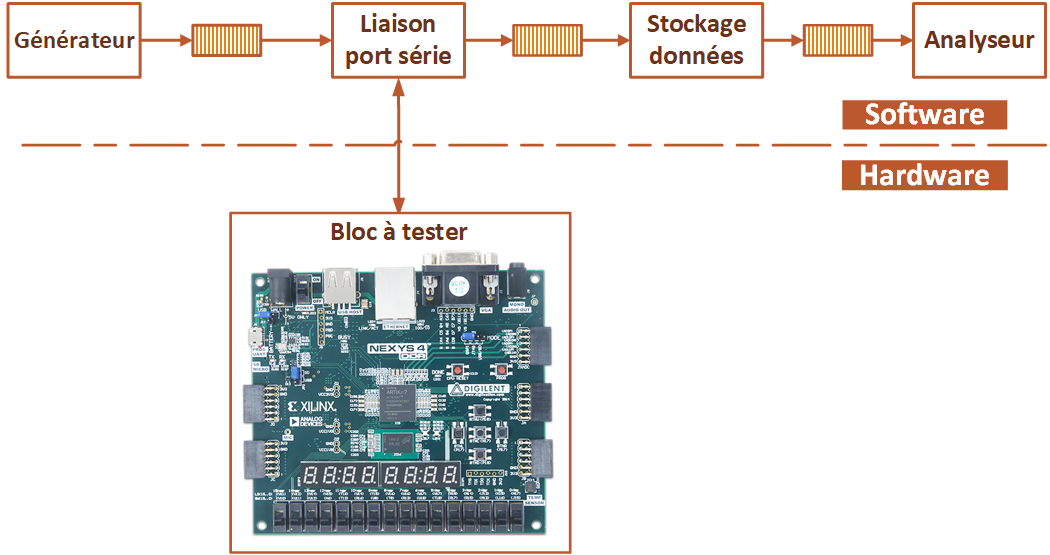
\includegraphics[width=\textwidth, keepaspectratio]{Dessin6.png}
		\caption{Environnement de test}
	\end{figure}
	\noindent On distingue ici deux parties essentielles :\\
	\begin{itemize}
		\item[\textbullet] la partie \textit{software} : elle se déroule sur un ordinateur, sous \textit{Vivado HLS} par exemple, et permet de lancer une simulation,\\
		\item[\textbullet] la partie \textit{hardware} : elle représente la carte Nexys 4 reliée en USB sur le port série de l'ordinateur, elle contient également l'implémentation du bloc IP à tester.\\
	\end{itemize}

	Avant de tester les chaînes globales développées en SystemC, les blocs réalisant la racine carrée ainsi que la puissance au carré ont notamment été implémentés sur FPGA. Pour ce faire, le bloc "\textit{Générateur}" permet de venir lire les données d'entrée stockées dans un fichier texte, que ce soit les valeurs extraites du signal biomédical ou bien des valeurs plus rudimentaires pour tester la racine carrée. Après passage dans une FIFO, les données sont envoyées sur le port série et traitées sur le FPGA. Ce dernier contient l'IP que l'on souhaite tester en \textit{hardware}, la racine carrée par exemple, et renvoie les données sortantes vers le bloc "\textit{Stockage données}". Ce bloc écrit alors les données calculées sur le FPGA dans un fichier texte. Comme expliqué en 2.2, les données contenues dans une FIFO doivent être consommées, c'est pourquoi le bloc "\textit{Analyseur}" se contente de venir lire dans la FIFO, pour fermer la chaîne de test.  \\ \\
	\indent En ce qui concerne l'échange de données entre la partie \textit{software} et le FPGA, le module de communication utilisant l'UART et développé par Yannick Bornat a été utilisé. Cependant, les deux chaînes précédemment décrites manipulent des données de type \textit{float}, donc sur 32 bits, tandis que l'UART ne reçoit et renvoie que des données sur 8 bits. Pour palier à cette incompatibilité, des \textit{wrappers} ont été décrit en SystemC selon le modèle présenté en Figure X. Le \textit{wrapper} IN reçoit les données de la partie \textit{software} sur 32 bits et les envoie par parquets de 8 bits à l'UART, tandis que le \textit{wrapper} OUT fait l'opération inverse et attend de recevoir quatre paquets de 8 bits pour reformer et renvoyer la donnée voulue sur 32 bits au bloc "\textit{Stockage données}" présenté en Figure X. Ces deux wrappers ont alors été synthéthisés et exportés en tant qu'IP avec le bloc à tester.  
	\begin{figure}[H]
		\centering
		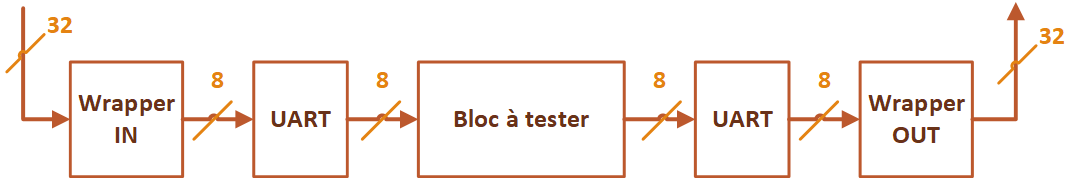
\includegraphics[width=\textwidth]{Dessin7.png}
		\caption{UART Wrappers}
	\end{figure}   

	Lorsque les différents blocs ont été validés un à un sur cet environnement de test, les deux chaînes ont pu successivement être implémentées sur FPGA. Leur validation est, quant à elle, passée par une comparaison entre les données traitées et celles de référence obtenues après développement en VHDL de Yannick Bornat. La principale difficulté de cette démarche d'implémentation \textit{hardware} résidait dans l'envoi et la réception des données entre la chaîne de simulation et la carte Nexys 4. En effet, le goulot d'étranglement se trouve dans la communication avec l'UART qui attend de recevoir une donnée avant d'en transmettre une autre. Une fois cette notion appréhendée il a été possible de vérifier le fonctionnement de n'importe quels blocs.
\newpage
\section{Résultats}
	Après simulation et implémentation de l'ensemble des blocs et de la chaine de filtrage, il est necessaire de comparer les sorties afin de verifier la similitude des deux systèmes et en noter les différences.
\subsection{Comparaison des sorties}
A l'aide d'un code sous matlab, la sortie du système simulé est comparé aux données fournise par monsieur Bornat.
L'idée ici est de mettre en avant le bon fonctionnement du système en montrant l'equivalence des résultats de sortie avec ceux du système de référence.
Les indices des pics détéctés sont donc extrait d'un fichier texte contenant les sorties du système et comparé avec les indices contenus dans le fichier de référence.
La différence entre les indices sources et références sont enregistrés et si celui-ci dépasse les 50 echantillons, la sortie source sera considéré comme une erreur. 
\begin{figure}[H]
	\centering
	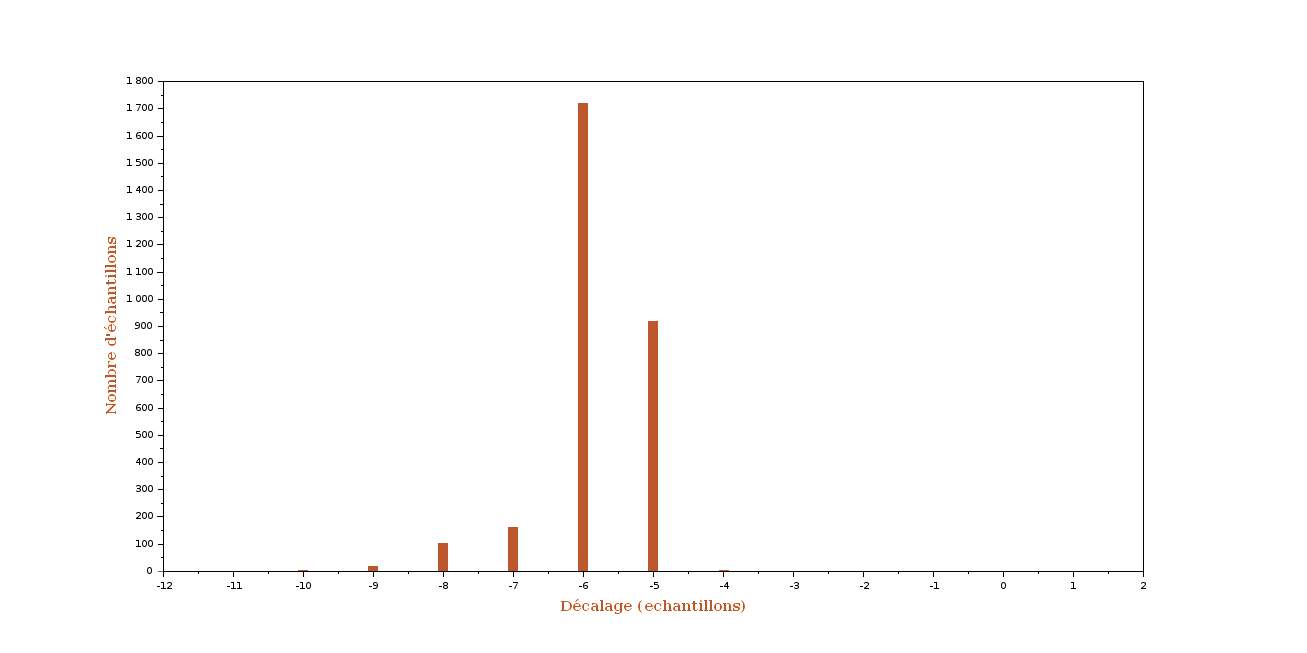
\includegraphics[scale=0.3, keepaspectratio]{ResultatSim.png}
	\caption{\textit{Représentation du décalage de détéction entre le système simulé et la référence}}
\end{figure}
La figure X montre les décalages retrouvés sur l'ensemble des pics fournit dans le fichier source. Le système montre 65 erreurs sur les 2990 pics ce qui correspond à un ratio de $98\%$ de similitude.
Enfin, comme le montre la figure, les pics sont détécté entre 4 et 9 echantillons avant l'indice présent dans le fichier de référence. Ceci s'expliquer par une différence de moyen de détéction entre la source et le système de référence.
En effet, le pic biologique étant plus large qu'un simple échantillon, l'abscence de système anti-rebond dans notre simulation explique parfaitement ce décalage.
Nous avons donc considéré que les deux systèmes était équivalent en terme de comportement.
\newpage
\subsection{Ressources utilisées}
Après avoir validé le comportement de notre chaine, l'important maintenant est de comparer l'utilisation des ressources à l'aide du rapport de synthèse fournit par HLS.
Cette comparaison est faite sans utiliser de moyen d'optimisation afin de juger des performances du systemC. Néanmoins, il va de soit que les performances d'un système écrit par des etudiants seront nettement moins bonnes que celle obtenues sur un système ecrit par un utilisateur expérimenté du VHDL.
\begin{table}[h]
	\centering
	\begin{tabular}{|
	>{\columncolor[HTML]{F2B25C}}c |
	>{\columncolor[HTML]{FFFFFF}}r |
	>{\columncolor[HTML]{FFFFFF}}r |
	>{\columncolor[HTML]{FFFFFF}}c |}
	\hline
	\cellcolor[HTML]{BD591C} & \multicolumn{1}{c|}{\cellcolor[HTML]{F2B25C}SystemC (64 channels)} & \multicolumn{1}{c|}{\cellcolor[HTML]{F2B25C}VHDL} & \cellcolor[HTML]{F2B25C}Difference \\ \hline
	LUT                      & 5632                                                               & X                                                 & {\color[HTML]{CB0000} XXX}         \\ \hline
	DSP                      & 26                                                                 & 1                                                 & {\color[HTML]{CB0000} +2500\%}     \\ \hline
	FF                       & 2789                                                               & X                                                 & {\color[HTML]{CB0000} XXX}         \\ \hline
	RAM (512*32bits)         & 5                                                                  & 2                                                 & {\color[HTML]{CB0000} +150\%}      \\ \hline
	Development Time (hours) & 35                                                                 & 50                                                & {\color[HTML]{009901} -30\%}       \\ \hline
	\end{tabular}
	\caption{Utilisation des ressources des deux systèmes}
	\end{table}
	La table XX récapitule l'utilisation des ressources fournit pour notre système par HLS et par monsieur Bornat pour le sien. N'ayant pas sentit l'utilité de s'interesser aux LUT et aux bascules flip-flop, ces données ne nous ont pas été communiquées.
Il y a trois points interessants dans ce tableau : 
\begin{itemize}
	\item[•] \textbf{Le nombre de DSP} utilisés est nettement plus élevé. Cette différence s'explique par l'utilisation de nombres flottants sur 32 bits contre des nombres à virgule fixe sur 16 bits dans le système de référence. De plus, l'utilisation d'un seul DSP dans le système de référence montre la volonté de monsieur Bornat de limiter le nombre de DSP utilisés ce qui n'a pas été notre cas.
	\item[•] \textbf{Le nombre de RAM} utilisés qui découle de l'allocation par HLS d'un bloc RAM pour chaque tableau présent dans notre code. Une fois de plus, cette valeur se trouve être plus élevée que celle du système de référence.
	\item[•] \textbf{Le temps de développement} quant à lui est $30\%$ inférieur dans le cadre d'un développement en systemC par rapport à une description en VHDL.
\end{itemize}
Ces données nous montre que l'utilisation du systemC via HLS pour la synthèse de système permet un gain de temps non négligeable. L'optimisation des ressources est quant à elle possible en ajoutant simplement quelques directives pour la synthèse et n'a pas été traité ici. 
\newpage
\section{Conclusion}

\end{document}


